\documentclass[UTF8]{ctexart}
\usepackage{amsmath}
\usepackage{amssymb}
\usepackage{booktabs}
\usepackage{background}
\usepackage{caption,subcaption}
\usepackage{enumitem}
\usepackage{fancyhdr}
\usepackage{float}
\usepackage{fontspec}
%\usepackage{fourier}
\usepackage{geometry}
\usepackage{hyperref}
\usepackage{imakeidx}
\usepackage{listings}
\usepackage{pifont}
\usepackage{tcolorbox}
\tcbuselibrary{breakable}
\usepackage{tikz}
\usetikzlibrary{arrows.meta, positioning, shapes.geometric, calc}
\usepackage{xcolor}

\geometry{a5paper, top=0.1cm, left=1cm, right=1cm, bottom=1cm, footskip=0.1cm}
\setCJKmainfont[BoldFont={汉仪文黑-85W},ItalicFont={方正苏新诗柳楷简体}]{汉仪文黑-55W}
\setfontfamily\Issue{Century Schoolbook}
\setfontfamily\Genshin{Genshin Teyvat Lingua Franca}
\newCJKfontfamily\TitleFont{思源宋体 CN Heavy}
\newfontfamily\timesnewroman{Times New Roman}
\captionsetup{font=small, labelfont=bf}

\pagestyle{fancy}
\fancyhf{}
\cfoot{\sffamily\footnotesize{-\ \thepage\ -}}
\CTEXsetup[format={\bfseries\large\color{darkcyan}}]{subsection}
%\CTEXsetup[format = {\centering\bfseries\large}, beforeskip = 3pt, afterskip = 3pt]{section}

\colorlet{darkcyan}{cyan!50!black}
\newcommand\Black[1]{\textcolor[gray]{0.3}{#1}}
\newcommand\Brown[1]{\textcolor[HTML]{998A4E}{#1}}
\newcommand\Emph[1]{\colorbox{green!10}{\textcolor{green!30!black}{#1}}}
\newcommand\Notes[1]{\textcolor{yellow!50!black}{\small #1}}
\newcommand\Example[1]{\textcolor{cyan!70!black}{\small #1}}


% -----------------本文档专用-----------------
\setlist{itemsep=0pt, parsep=0pt}
\newcommand\kw[1]{\textsc{#1}} % key word 关键字
\hypersetup{pdfborder=0 0 0}
\lstset{
    basicstyle=\small\ttfamily, %注意行末有逗号!
    keywordstyle=\bfseries\color{blue!70!black}\ttfamily\scshape,
    commentstyle=\color{cyan!90!black},
    stringstyle=\color{green!40!black},
    columns=flexible,
    numbers=left,
    numberstyle=\footnotesize,
    escapechar=`,
    frame=shadowbox,
    %rulesepcolor=\color{red!20!blue!20!green!20}
    backgroundcolor=\color{cyan!5!white},
    language = SQL,
    tabsize = 4,
    breaklines = true,
}
% ---------------------------------------------

\newcommand\IssueNumber{54}
\newcommand\Date{2025-5-12}
%\newcommand\Contributer{@金光日}
\newcommand\Subject{数据库系统原理}
%\newcommand\Source{2023 考研 408 真题}


\begin{document}
\backgroundsetup{contents=
\includegraphics{上半示例.png}, center, scale=1, angle=0, opacity=1}
\BgThispage
\begin{center}
%{\scriptsize\Issue \textcolor[HTML]{C8BA83}{\Genshin WEEKLY TIPS}}
\phantom{...}

{\Large\textcolor{brown!40!white}{\makebox[10cm][s]{\Genshin WEEKLY KNOWLEDGE TIPS}}}

\vspace{-2em}

{\Huge\bfseries\TitleFont \Black{知\ 识\ 小\ 料}}


\vspace{-0.1cm}
{\footnotesize \Brown{「电计 2203 班」周常规知识整理共享}}
\end{center}

\vspace{-0.5cm}


\begin{figure}[H]
\hspace{1cm}
\begin{minipage}[t]{0.3\textwidth}
\centering
    \Brown{\Genshin ISSUE}

    \vspace{-0.6cm}
    \Huge \Issue\slshape\bfseries\Black{\IssueNumber}
\end{minipage}
\hfill
\begin{minipage}[t]{0.3\textwidth}
\centering
\vspace{-0.1cm}
    \Brown{日期:\Date} \\
%\vspace{-0.1cm}
%    \Brown{贡献者:\Contributer} \\
%\vspace{0.1cm}
    \Brown{学科:\Subject} \\
%\vspace{-0.1cm}
%    \Brown{来源:\Source} \\
\end{minipage}
\hspace{0.8cm}
\end{figure}

{\color{darkcyan} 本文档对课程内常见 SQL 语法作出整理。}

\begin{quote}
    \small 基本规则:
\begin{enumerate}[itemsep=0pt,parsep=0pt]
     \item SQL 不区分大小写;
     \item SQL 语句末尾以分号结束,缩进不影响结果;
     \item SQL 注释以两个减号开头,例如「\verb!-- 注释内容!」。
\end{enumerate}
\end{quote}


\tableofcontents

\newpage
\backgroundsetup{contents=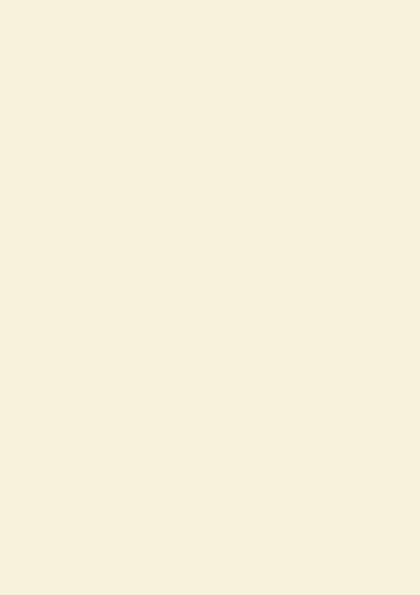
\includegraphics{空白示例.png}, center, scale=1, angle=0, opacity=1}
\BgThispage
\section{数据定义}
数据定义语句包括 \kw{Create}、\kw{Drop}、\kw{Alter} 语句,一般为对数据库、表、视图等宏观概念的定义。

\subsection{Create 创建}

\paragraph{创建表}
以下语句用于创建表。
\begin{lstlisting}
Create Table 表名(
    列名  数据类型    列级完整性约束,
    列名  数据类型    列级完整性约束,
    ...
    列名  数据类型    列级完整性约束,
表级完整性约束);
\end{lstlisting}

\begin{lstlisting}[backgroundcolor=\color{white}]
Create Table Course(
    Cno Char(4) Primary Key,
    Cname Char(40),
    Cpno Char(4),
    Ccredit Smallint,
    Foreign Key (Cpno) References Course(Cno)
);
\end{lstlisting}
\begin{itemize}
    \item Primary Key 表示主键约束;
    \item Foreign Key 表示外键约束,其中的 References 指向对应表的对应主属性。
\end{itemize}

\paragraph{创建模式}
以下语句用于创建模式,较少使用。
\begin{lstlisting}
Create Schema 模式名 Authorization 用户名;
\end{lstlisting}


\paragraph{创建视图}
以下语句用于创建视图。
\begin{lstlisting}
Create View 视图名(列, 列, ..., 列) As
    子查询
[With Check Option];
\end{lstlisting}
With Check Option 若被使用,则在视图增、删、改元组时会自动加上子查询中的条件。

\begin{lstlisting}[backgroundcolor=\color{white}]
Create View CS_Student_View(Sno, Sname, Sage) As
    Select Sno, Sname, Sage From Student Where Sdept = 'CS'
With Check Option;
\end{lstlisting}
建立计算机系学生的学号、姓名、年龄视图,其中对视图增、删、改元组时会自动加上 \verb!Sdept = 'CS'! 的条件。

\paragraph{创建索引}
以下语句用于创建索引。
\begin{lstlisting}
Create [Unique] [Cluster] Index 索引名
On 表名(列 [次序], 列 [次序], ..., 列 [次序])
\end{lstlisting}

\begin{lstlisting}[backgroundcolor=\color{white}]
Create Unique Index Student_Index
On Student(Sno Desc);
\end{lstlisting}
对学生表按照学号列降序建立一个唯一索引。


\subsection{Drop 删除}
\paragraph{删除表} 以下语句用于删除表。Restrict 表示限制条件,Cascade 表示级联删除,默认 Restrict(下同)。
\begin{lstlisting}
Drop Table 表名 [Restrict/Cascade];
\end{lstlisting}

\begin{lstlisting}[backgroundcolor=\color{white}]
Drop Table Student Cascade;
\end{lstlisting}

\paragraph{删除模式} 以下语句用于删除模式。删除模式会将其定义的表也删除。
\begin{lstlisting}
Drop Schema 模式名 [Restrict/Cascade];
\end{lstlisting}

\paragraph{删除视图}以下语句用于删除视图。
\begin{lstlisting}
Drop View 视图名 [Restrict/Cascade];
\end{lstlisting}

\paragraph{删除索引}以下语句用于删除索引。
\begin{lstlisting}
Drop Index 索引名;
\end{lstlisting}

\subsection{Alter 修改}
\paragraph{修改表} 以下语句用于修改表中列。几个语句之间是独立的。
\begin{lstlisting}
Alter Table 表名 Add Column 列名   数据类型    列级完整性约束;
Alter Table 表名 Drop Column 列名 [Cascade/Restrict];
Alter Table 表名 Alter Column 列名   数据类型 ;
\end{lstlisting}

\begin{lstlisting}[backgroundcolor=\color{white}]
Alter Table Student Add Column S_entrance Date Not Null; -- 新增入学时间列
Alter Table Student Drop Column Sage Cascade; -- 级联删除年龄列
Alter Table SC Alter Column Grade Int; -- 修改成绩列
\end{lstlisting}

以下语句用于修改表中的完整性约束。
\begin{lstlisting}
Alter Table 表名 Add 表级完整性约束;
Alter Table 表名 Drop Constraint 完整性约束名 [Cascade/Restrict];
\end{lstlisting}

\begin{lstlisting}[backgroundcolor=\color{white}]
Alter Table Student Add Unique(Sname); -- 增加姓名唯一性
Alter Table Student Drop Constraint sp_ibfk_1; -- 删除某个特定约束
\end{lstlisting}

\paragraph{修改索引} 以下语句用来对索引重命名。
\begin{lstlisting}
Alter Index 旧索引名 Rename To 新索引名;
\end{lstlisting}

\section{数据操纵}
数据操纵语句包括 \kw{Insert}、\kw{Delete}、\kw{Update} 语句,一般为对元组等微观概念的操纵。

\subsection{Insert 数据插入}
\paragraph{插入元组} 以下语句用于插入元组。数据的顺序需要与列的顺序一致(而列的顺序可以重排)。
\begin{lstlisting}
Insert Into 表名(列, 列, ..., 列)
    Values (数据, 数据, ..., 数据);
\end{lstlisting}

\begin{lstlisting}[backgroundcolor=\color{white}]
Insert Into Student(Sno, Sname, Sage, Ssex, Sdept) Values
    ("22001", "小明", 20, "男", "CS"),
    ("22002", "小红", 19, "女", "IS"),
    ("22003", "小刚", 21, "男", "AI");
\end{lstlisting}

\paragraph{插入子查询结果} 以下语句通过子查询结果用于插入元组。较少使用。
\begin{lstlisting}
Insert Into 表名(列, 列, ..., 列)
    子查询;
\end{lstlisting}

\begin{lstlisting}[backgroundcolor=\color{white}]
Insert Into Student2(Sno, Sname, Sage)
    Select Sno, Sname, Sage From Student Where Sdept = "CS";
\end{lstlisting}

\subsection{Delete 数据删除}
\begin{lstlisting}
Delete From 表名 Where 条件;
\end{lstlisting}

\begin{lstlisting}[backgroundcolor=\color{white}]
Delete From SC Where Sno In (
    Select Sno From Student Where Sdept = 'IS' );
\end{lstlisting}
删除信息系学生的选课记录。

\subsection{Update 数据修改}
Update 可以用于表中数据修改,也可以用于视图中数据修改。

\begin{lstlisting}
Update 表名/视图名
Set 列名=表达式, 列名=表达式, ... , 列名=表达式
Where 条件;
\end{lstlisting}

\begin{lstlisting}[backgroundcolor=\color{white}]
Update Student
Set Sage=Sage+2, Sdept="CS"
Where Sno="22001";
\end{lstlisting}

\section{数据查询}
\subsection{Select 查询语句}
数据查询语句也即 \kw{Select} 语句,用途十分广泛,复习时以教师课件为准。

\paragraph{版本1}(基础款)
\begin{lstlisting}
Select 目标列
From 表名/视图名
Where 条件;
\end{lstlisting}

\begin{lstlisting}[backgroundcolor=\color{white}]
Select * From Student Where Sage>=20;
\end{lstlisting}
查询年龄大于等于20岁的学生的全部信息。

\paragraph{版本2}(带排序)
\begin{lstlisting}
Select 目标列
From 表名/视图名
Where 条件
Order By 排序属性 [Asc/Desc];
\end{lstlisting}

\begin{lstlisting}[backgroundcolor=\color{white}]
Select * From Student Where Sdept="CS" Order By Sage Desc;
\end{lstlisting}
查找计算机系学生的全部信息,按照年龄降序排列。

\paragraph{版本3}(指定去重)
\begin{lstlisting}
Select [All/Distinct] 目标列
From 表名/视图名
Where 条件;
\end{lstlisting}

\begin{lstlisting}[backgroundcolor=\color{white}]
Select All Sno From SC Where Grade>=60;
\end{lstlisting}
在选课表中查询及格学生的学号,同一学号输出次数取决于及格科目数。如果把其中的 All 换成 Distinct,那么同一学号仅输出一次。

\paragraph{版本4}(带Group by子句)
\begin{lstlisting}
Select 目标列
From 表名/视图名
Where 全局条件
Group By 列名
Having 组内条件(可能采用聚集函数);
\end{lstlisting}

\begin{lstlisting}[backgroundcolor=\color{white}]
Select Sno From SC Where Grade>=60
Group By Sno Having Count(*)>=3;
\end{lstlisting}
查询及格课程数大于等于 3 门的学生的学号。此查询的过程是:
\begin{enumerate}
    \item 先在 SC 表中选出 $\mathrm{Grade\geqslant 60}$ 的元组,排除不及格元组;
    \item 再对这些元组按照 Sno 进行分组,相同 Sno 的分成一组;
    \item 随后将一组内记录条数 $\geqslant 3$ 条的组号(即Sno)筛选出来,返回结果。
\end{enumerate}


\begin{lstlisting}[backgroundcolor=\color{white}]
Select Sno,Count(*),Avg(Grade) From SC Where Grade>=60
Group By Sno Having Avg(Grade)<80;
\end{lstlisting}
查询均分小于 80 分的学生的学号,仅统计及格科目。此查询的过程是:
\begin{enumerate}
    \item 先在 SC 表中选出 $\mathrm{Grade\geqslant 60}$ 的元组,排除不及格元组;
    \item 再对这些元组按照 Sno 进行分组,相同 Sno 的分成一组;
    \item 随后将一组内平均分小于 80 分的组号(即Sno),以及及格科目数和平均分筛选出来,返回结果。
    \item 需要注意的是:计算平均分之前,就已经把不及格的科目排除在外了。
\end{enumerate}


\paragraph{版本5}(外连接)
\begin{lstlisting}
Select 目标列 From 左表
Left/Right Outer Join 右表 On(连接约定)
Where 条件;
\end{lstlisting}

\begin{lstlisting}[backgroundcolor=\color{white}]
Select Student.Sno, Sname, Ssex, Sage, Sdept, Cno, Grade From Student
Left Outer Join SC On(Student.Sno = SC.Sno)
Where Sdept='CS';
\end{lstlisting}
将 Student 表的学号、姓名、性别、年龄、院系与 SC 表的课程号、成绩连接起来,使用左外连接(即使 Student 表中有的元组在 SC 表没有任何值,也必须保留,这时的 Cno 和 Grade 字段返回 NULL),且仅限于计算机专业。


\paragraph{版本6}(带别名)
\begin{lstlisting}
Select 目标列 别名(或不止一个)
From 表名 别名, 表名 别名, ..., 表名 别名
Where 条件;
\end{lstlisting}

\begin{lstlisting}[backgroundcolor=\color{white}]
Select S1.Sno "学号", S1.Sname "姓名", S1.Sage "年龄"
From Student S1, Student S2
Where S1.Sdept = S2.Sdept And S2.Sname = "刘晨";
\end{lstlisting}
查询与刘晨在同一个系学习的学生,这里的 S1,S2 即为 Student 的别名,「学号」、「姓名」和「年龄」是查询返回结果的别名。这个例子其实是自身连接。


\paragraph{版本7}(集合查询)
\begin{lstlisting}
子查询甲
Intersect/Union/Except
子查询乙;
\end{lstlisting}

\begin{lstlisting}[backgroundcolor=\color{white}]
Select * From Student Where Sage=20
Intersect
Select * From Student Where Sdept="CS";
\end{lstlisting}
查询计算机系的 20 岁学生的全部信息。

\subsection{条件的千变万化}
条件语句是千变万化的,其中可能的变体有:
\begin{itemize}
    \item 比较:\verb|= > < >= <= != <>|,可能添加 Not
    \item 确定范围:(Not) Between ... And ...
    \item 确定集合:(Not) In
    \item 字符匹配:(Not) Like,匹配字符串中 \verb!%! 代表任意个字符(包括 0 个),\verb!_! 代表 1 个字符。可能使用 Escape 转码字符。
    \item 空值:Null
    \item 逻辑:And、Or、Not
    \item 量词:All、Any
    \item 存在谓词:(Not) Exists
\end{itemize}

\section{数据控制}
数据控制语句包括 \kw{Grant}、\kw{Revoke} 语句,一般为对用户数据库权限的管理。默认情况下,作出数据控制的角色是数据库管理员(DBA)或者其他有权限操作的用户。

\subsection{Grant 授予权限}
\begin{lstlisting}
Grant 权限(或为 All Privileges)
On 对象类型 对象名
To 用户(或为 Public)
[With Grant Option];
\end{lstlisting}

\begin{lstlisting}[backgroundcolor=\color{white}]
Grant Select, Update(Sno)
On Table SC
To User1
With Grant Option;
\end{lstlisting}
将对选课表的查询和修改学号权限授予用户 1,且允许其再授予二级权限。

\subsection{Revoke 撤回权限}
\begin{lstlisting}
Revoke 权限(或为 All Privileges)
On 对象类型 对象名
From 用户(或为 Public)[Cascade/Restrict]
\end{lstlisting}

\begin{lstlisting}[backgroundcolor=\color{white}]
Revoke All Privileges
On Table SC
From User1;
\end{lstlisting}
撤回用户 1 对选课表的全部权限。注意 Revoke 语句用介词 From,而 Grant 语句用介词 To。

\section{约束完整性命名}
Constraint (约束完整性)是一种数据对象,一般在插入或删除操作中使用到。本节相当于给定义的约束完整性显式命名,其格式为
\begin{lstlisting}
Constraint  约束条件名   约束条件内容
\end{lstlisting}
其中约束条件内容包括 Not Null、Unique、Primary Key、Foreign Key、Check 等。

\paragraph{插入操作的完整性命名} 举个例子:
\begin{lstlisting}[backgroundcolor=\color{white}]
Create Table Student(
    Sno Numeric(6)
        Constraint C1 Check (Sno Between 90000 And 99999),
    Sname Char(20)
        Constraint C2 Not Null,
    Sage Smallint
        Constraint C3 Check (Sage>0 And Sage<30),
    Ssex Char(2)
        Constraint C4 Check (Ssex in ("男","女")),
    Constraint C5 Primary Key(Sno) -- 表级完整性约束
);
\end{lstlisting}

\paragraph{修改操作的完整性命名} 举两个例子:
\begin{lstlisting}[backgroundcolor=\color{white}]
Alter Table Student Drop Constraint C2; -- 删除 C2 即「名字非空」完整性
Alter Table Student Add Constraint C2 Not Null; -- 再加回来
\end{lstlisting}

\section{触发器}
触发器也称为「事件—条件—动作」规则。

\paragraph{创建触发器} 在一个表定义触发器的格式如下:
\begin{lstlisting}
Create Trigger 触发器名
Before/After 触发事件 On 表名
Referencing New/Old Row As 变量
For Each Row/Statement
When(触发条件)
    触发动作体
\end{lstlisting}
其含义为:
\begin{enumerate}
    \item 如果在某个表上发生了某种触发事件(Update、Insert 等),那么在触发事件之前(或之后),需要执行触发动作体;
    \item 显式定义旧元组与新元组为某一变量,以便触发动作体使用该变量;
    \item 在触发时,对于每一行(或每条语句),若触发条件为真,则执行一次触发动作体。
\end{enumerate}

\begin{lstlisting}[backgroundcolor=\color{white}]
Create Trigger Salary_Trigger
Before Insert Or Update On Teacher
Referencing New Row As NewTuple
For Each Row
Begin
    If NewTuple.Job="教授" And NewTuple.Sal<4000 Then
        NewTuple.Sal=4000;
    End If;
End;
\end{lstlisting}
该触发器会在插入或更新教师表之前生效,如果教授的工资低于 4000 元则自动转换为 4000 元。这个例子仅供演示,MySQL 不直接支持这种写法。 

\paragraph{删除触发器} 删除一个触发器用 Drop 即可实现。
\begin{lstlisting}
Drop Trigger 触发器名 On 表名;
\end{lstlisting}

\section{事务操作}
事务是数据库的不可分割的基本单位,具有原子性、一致性、隔离性、持续性。事务定义语句一般如下:
\begin{lstlisting}
Begin Transaction;
若干条语句;
Commit/Rollback;
\end{lstlisting}

在 MySQL 中,开头语句为 \verb!Start Transaction;!。

\begin{lstlisting}[backgroundcolor=\color{white}]
Start Transaction;
Update Student Set Sage=Sage-1 Where Sdept='CS';
Select * From Student;
Rollback;
Select * From Student;
\end{lstlisting}
对计算机系学生的年龄减 1,然后回退。回退以后的数据还原至事务开始前的状态,相当于在回退前对计算机系学生的年龄加 1。这是 MySQL 语法,开头语句用 \verb!Begin! 还是 \verb!Start! 随数据库语法而确定。


\backgroundsetup{contents=
\includegraphics{下半示例.png}, center, scale=1, angle=0, opacity=1}
\BgThispage
\end{document} 